%
%
%
\chapter{Einf�hrung und �berblick}\label{sec:Einf�hrung}
%
%
%
Zu Beginn einer jeden Neuentwicklung steht eine Idee. Um die Realisierbarkeit dieser Idee zu �berpr�fen versucht man sie mittels eines mathematischen Modells zu beschreiben, und eventuell auftretende Probleme abzusch�tzen. Die mathematische Beschreibung l�sst sich dann mit Programmen wie MATLAB in der Simulation �berpr�fen. 

In unserem Fall ist der Ausgangspunkt das in Abbildung \ref{abb:Blockschaltbild01} dargestellte Blockschaltbild. In diesem werden die beiden obersten Abstraktionsebenen der Funktion dargestellt. \begin{figure}[h]
	\centering 
%	\psfrag{01}{MATLAB Workspace}
%	\psfrag{02}{Command-Window} 
%	\psfrag{03}{Command-History}
	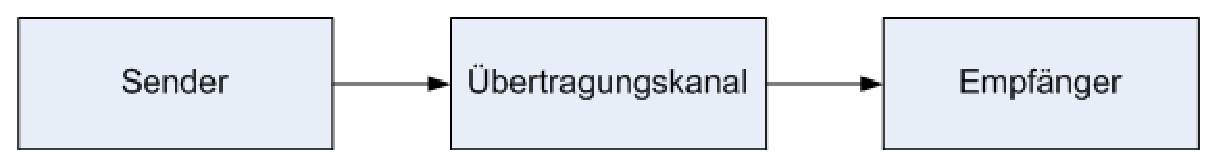
\includegraphics[width=11cm]{bilder/einf�hrung/blockschaltbild01}
	\caption{Blockschaltbild �bertragungsstrecke}
	\label{abb:Blockschaltbild01}
\end{figure}
\paragraph{Sender}Der Bitstromgenerator erzeugt eine (vorerst beliebige) Folge von Nullen und Einsen. Vom Sender werden jetzt zwei freilaufende Sinussignale erzeugt, von denen das eine mit dem Bitstrom und das andere mit dem negierten Bitstrom multipliziert wird. Die resultierenden Signale werden additiv �berlagert. Jetzt wird f�r eine Null die Sinusschwingung des Generators 2 und f�r eine Eins die Schwingung des Generators 1 ausgegeben. 
\paragraph{Kanal}
\paragraph{Empf�nger}Im Empfangsteil sollen die beiden Signale mittels zweier Bandp�sse wieder separiert werden. Danach wird mittels der H�llkurvendemodulatoren und der anschliessenden Gl�ttung durch die beiden Tiefp�sse das urspr�ngliche Signal wieder rekonstruiert. 

\medskip Ziel dieses Kapitels ist es nun, ein komplettes (und funktionsf�higes) Modell der �bertragungsstrecke in MATLAB aufzubauen und die Funktion der Schaltung zu validieren.

%
%
%
\chapter{Sender}\label{sec:Sender}
%
%
%


%
%
\section{Erzeugen einer zuf�lligen Bitfolge}\label{subsec:Bitfolge}
%
%


%
%
\section{Erzeugen der Tr�gerschwingungen}\label{subsec:Tr�gerschwingungen}
%
%

%
\subsection{Grundlagen}\label{subsec:Grundlagen_Signalgeneration}
%

%
\subsection{Programmierung in MATLAB}\label{subsec:Siggen_programmierung}
%



%
%
%
\chapter{Empf�nger}\label{sec:Empf�nger}
%
%
%


%
%
\section{Filterdesign}\label{subsec:Filterdesign}
%
%


%
\subsection{Grundlagen digitaler Filter}\label{subsec:digitalefilter}
%


%
\subsection{Entwurf in MATLAB}
%


%
%
\section{H�llkurvendemodulation}\label{subsec:H�llkurvendemodulation}
%
%


%
%
\section{Problematik Floating-Point / Fixed-Point}\label{sec:floating_fixed_point}
%
%

